%Общий объем раздела 15-25 стр. (x2, если разделы объединены)
% L2-регуляризация, нормировка входа и цветной ВАУ


\section{Описание разработанного программного обеспечения и экспериментальные исследования}

В рамках данной работы были реализованы три модели нейронных сетей для стегоанализа изображений в оттенках серого: GNCNN~\cite{GNCNN}, нейронная сеть с двумя свёрточными слоями~\cite{FrenchCNN} и комбинированная нейронная сеть. Впервые были получены свёрточные ИНС для стегоанализа цветных изображений путём модификации вышеперечисленных моделей. Также была произведена оценка различающей способности данных нейронных сетей.

\subsection{Структура разработанного программного обеспечения}

Модели нейронных сетей реализованы на языке программирования Python в виде шести интерактивных тетрадей IPython Notebook~\cite{ipynb} и протестированы с использованием интерпретатора Python~3.5.2. Реализация математического аппарата нейронных сетей предоставлена библиотеками Keras~2.2.4~\cite{Keras} и TensorFlow~1.13.1~\cite{TensorFlow}. Для отображения графиков процесса обучения использовалась библиотека livelossplot~0.3.4~\cite{livelossplot}.

Фильтр предварительной обработки для GNCNN и комбинированной нейронной сети был реализован в виде отдельного приложения на языке программирования C++. Также для проведения эксперимента был реализован стеганографический метод относительной замены коэффициентов дискретного косинусного преобразования (ДКП) Коха и Жао.

Архитектура модифицированной для работы с цветными изображениями нейронной сети GNCNN приведена на рис.~\ref{fig:GNCNNArchitecture}, нейронной сети с двумя свёрточными слоями --- на рис.~\ref{fig:FrenchCNNArchitecture}, комбинированной нейронной сети --- на рис.~\ref{fig:MixedCNNArchitecture}.

\begin{figure}[h]
\centering
\includegraphics[width=1\textwidth]{include/graphics/gncnn_color_architecture}
\caption{Архитектура GNCNN}
\label{fig:GNCNNArchitecture}
\end{figure}

\begin{figure}[!htb]
\centering
\includegraphics[width=1\textwidth]{include/graphics/french_color_architecture}
\caption{Архитектура сети с двумя свёрточными слоями}
\label{fig:FrenchCNNArchitecture}
\end{figure}

\begin{figure}[!htb]
\centering
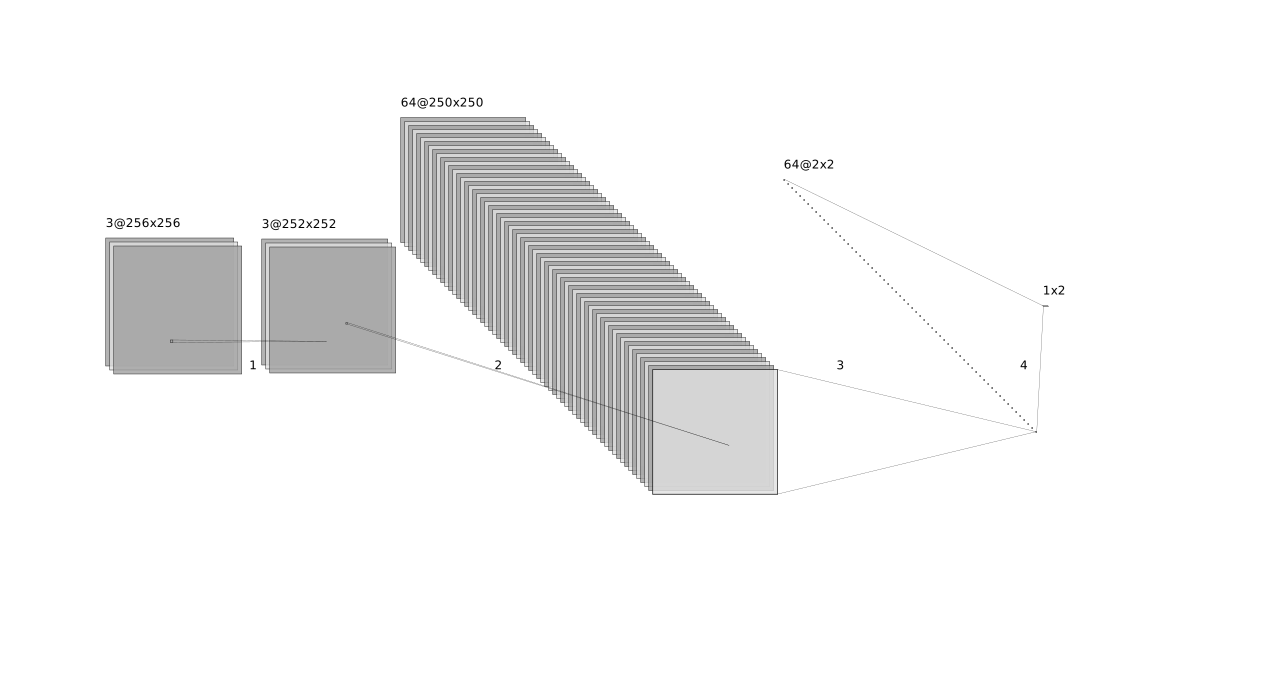
\includegraphics[width=1\textwidth]{include/graphics/mixed_color_architecture}
\caption{Архитектура комбинированной свёрточной сети}
\label{fig:MixedCNNArchitecture}
\end{figure}

Для обучения GNCNN было использовано значение параметра $ \sigma $ функции активации, равное 0,1, и метод обучения Adam со скоростью обучения 0,001, $ \beta_1 = 0,9 $, $ \beta_2 = 0,999 $. Для обучения нейронной сети с двумя свёрточными слоями и комбинированной нейронной сети использовался стохастический градиентный спуск со скоростью обучения 0,005.

\subsection{Результаты сравнительного исследования рассмотренных алгоритмов стегоанализа}

Целью проведения эксперимента было определение способности вышеописанных нейронных сетей различать пустые и заполненные различными стеганографическими методами контейнеры. Для заполнения использовалось следующее программное обеспечение:
\begin{itemize}
\item программная реализация метода создания цифровых водяных знаков на основе гетероассоциативных сжимающих преобразований (ГСП)~\cite{SirotaHIC};
\item собственная реализация метода относительной замены коэффициентов дискретного косинусного преобразования (ДКП) Коха и Жао~\cite{ZhaoKoch, KochZhao};
\item симулятор стеговстраивания с использованием алгоритма WOW~\cite{WOW}.
\end{itemize}

Для проведения эксперимента использовалась база данных изображений PPG-LIRMM-COLOR~\cite{PPG-LIRMM-COLOR}, состоящая из 10 000 изображений в разрешении 512×512 пикселей. База данных подверглась конвертации в формат изображений в оттенках серого с помощью утилиты ppmtopgm~\cite{ppmtopgm}. Затем из каждого изображения были вырезаны два фрагмента размером 256×256 пикселей: один из них использовался для обучения нейронной сети сжатия в составе реализации метода создания цифровых водяных знаков на основе ГСП, второй – для осуществления встраивания обученной сетью. В дальнейшем последний фрагмент также использовался для стеговстраивания с применением собственной реализации метода Коха и Жао и симулятора встраивания с использованием алгоритма WOW.

Таким образом, для обучения нейронных сетей были получены три выборки из 10 тыс. пустых и 10 тыс. заполненных одним из перечисленных стегоалгоритмов контейнеров. Такие же выборки были получены для цветных изображений из оригинальной базы.

Кроме того, были сформированы аналогичные выборки из 1 тыс. пустых и 1 тыс. заполненных контейнеров для оценки влияния объёма выборки на точность классификации.

Обучающая подвыборка составила 90~\% полученной выборки, валидационная --- 10~\% во всех случаях.

В рамках эксперимента было произведено сравнение реализаций методов стеговстраивания по средней среднеквадратической ошибке и среднему проценту восстановленных посредством стегоизвлечения данных (табл.~\ref{table:1} для контейнеров в оттенках серого и табл.~\ref{table:1Color} для цветных), а также обучение рассмотренных нейронных сетей с целью оценки их способности к классификации стегоконтейнеров валидационной подвыборки (табл.~\ref{table:2} для контейнеров в оттенках серого и табл.~\ref{table:2Color} для цветных).

Для каждого стегоалгоритма указан параметр, характеризующий мощность стеговоздействия. Для метода на основе гетероассоциативных сжимающих преобразований им является амплитуда встраивания $ A_m $, для алгоритма Коха и Жао – разность между коэффициентами ДКП $ p $, кодирующая различие между логическими нулём и единицей встраиваемой битовой последовательности, для алгоритма WOW – количество встроенных битов, делённое на количество пикселей в изображении, $ \alpha $.

\begin{table}[h!]
\centering
\caption{Сравнение методов встраивания в контейнеры в оттенках серого}
    \begin{tabular}{| l | l | l |}
    \hline
    Стегоалгоритм & MSE & Процент восстановленных данных \\ \hline
    На основе ГСП ($ A_m = 0,016 $) & 0,1334 & 97,23~\% \\ \hline
    Алгоритм Коха и Жао ($ p = 1 $) & 0,5775 & 99,78~\% \\ \hline
    WOW ($ \alpha = 0,4 $) & 0,0389 & – \\ \hline
%    \hline
    \end{tabular}
\label{table:1}
\end{table}

\begin{table}[h!]
\centering
    \begin{tabular}{| l | l | l |}
    \hline
    Стегоалгоритм & MSE & Процент восстановленных данных \\ \hline
    На основе ГСП ($ A_m = 0,016 $) & 0.0475 & 98,79~\% \\ \hline
    Алгоритм Коха и Жао ($ p = 1 $) & 0.1995 & 99,76~\% \\ \hline
    WOW ($ \alpha = 0,4 $) & 0.0129 & – \\ \hline
%    \hline
    \end{tabular}
\caption{Сравнение методов встраивания в цветные контейнеры}
\label{table:1Color}
\end{table}

Процент успешно извлечённых после стеговстраивания данных для алгоритма WOW не указан ввиду использования симулятора, не производящего сокрытия информации, а лишь изменяющего пиксели соответственно алгоритму встраивания.
\begin{landscape}

\begin{table}[h!]
\centering
    \begin{tabular}{| l | p{2cm} | p{2cm} | p{2cm} | p{2cm} | p{2cm} | p{2cm} |}
    \hline
    Стегоалгоритм & GNCNN (2 тыс.) & GNCNN (20 тыс.) & 2\=/хслойная НС (2 тыс.) & 2\=/хслойная НС (20 тыс.) & Комб. НС (2 тыс.) & Комб. НС (20 тыс.) \\ \hline
    На основе ГСП ($ A_m = 0,016 $) & 94,1~\% & 96,8~\% & 48~\% & 51,7~\% & 96~\% & 95,1~\% \\ \hline
    Алгоритм Коха и Жао ($ p = 1 $) & 50,7~\% & 93,1~\% & 100~\% & 99,8~\% & 100~\% & 99~\% \\ \hline
    WOW ($ \alpha = 0,4 $) & 50~\% & 49,6~\% & 85,5~\% & 96,3~\% & 92,5~\% & 95~\% \\ \hline
    \end{tabular}
\caption{Точность классификации контейнеров в оттенках серого}
\label{table:2}
\end{table}

\begin{table}[h!]
\centering
    \begin{tabular}{| l | p{2cm} | p{2cm} | p{2cm} | p{2cm} | p{2cm} | p{2cm} |}
    \hline
    Стегоалгоритм & GNCNN (2 тыс.) & GNCNN (20 тыс.) & 2\=/хслойная НС (2 тыс.) & 2\=/хслойная НС (20 тыс.) & Комб. НС (2 тыс.) & Комб. НС (20 тыс.) \\ \hline
    На основе ГСП ($ A_m = 0,016 $) & 53,7~\% & 99,5~\% & 50~\% & 50~\% & 82,5~\% & 100~\% \\ \hline
    Алгоритм Коха и Жао ($ p = 1 $) & 49,3~\% & 49,1~\% & 99,5~\% & 100~\% & 98~\% & 98,1~\% \\ \hline
    WOW ($ \alpha = 0,4 $) & 50~\% & 49,4~\% & 54,5~\% & 96,7~\% & 90~\% & 91,1~\% \\ \hline
    \end{tabular}
\caption{Точность классификации цветных контейнеров}
\label{table:2Color}
\end{table}
\end{landscape}

Из табл.~\ref{table:2} видно, что все три нейронные сети имеют практически одинаковую способность к различению пустых стегоконтейнеров и стегоконтейнеров, заполненных с помощью реализации метода Коха и Жао, на выборке из 20 тыс. изображений в оттенках серого.

Однако нейронная сеть с двумя свёрточными слоями оказалась неспособна успешно детектировать заполненные с помощью реализации метода на основе ГСП стегоконтейнеры, а GNCNN --- заполненные с применением симулятора встраивания WOW, в то время как комбинированная нейронная сеть одинаково хорошо справляется с обоими алгоритмами.

Объём выборки не возымел существенного влияния на точность классификации во всех случаях, кроме распознавания контейнеров, заполненных методом Коха и Жао, нейронной сетью GNCNN.

Из табл.~\ref{table:2Color} видно, что GNCNN хуже распознаёт цветные контейнеры, чем контейнеры в оттенках серого: для алгоритма на основе ГСП проявляется влияние объёма выборки, метод Коха и Жао перестаёт детектироваться вовсе. Различающая способность нейронной сети с двумя свёрточными слоями также начинает зависеть от объёма выборки для алгоритма WOW. Комбинированная нейронная сеть ухудшает свои показатели по сравнению со случаем контейнеров в оттенках серого, но точность классификации остаётся приемлемой.

Рис.~\ref{fig:GrayscalePlots} и ~\ref{fig:ColorPlots} иллюстрируют процесс обучения нейронных сетей. Видно, что комбинированная нейронная сеть зачастую имеет более гладких характер кривых для валидационной подвыборки.

\begin{figure}[p]
    \centering

    \begin{subfigure}{\textwidth}
        \includegraphics[width=\textwidth]{include/graphics/experimental_plots/grayscale/gncnn_hic}
                    \caption{GNCNN (ГСП)}
    \end{subfigure}

    \begin{subfigure}{\textwidth}
        \includegraphics[width=\textwidth]{include/graphics/experimental_plots/grayscale/mixed_hic}
                    \caption{Комб. НС (ГСП)}
    \end{subfigure}

   \caption{Графики процесса обучения в случае контейнеров в оттенках серого}
    \label{fig:GrayscalePlotsHIC}
\end{figure}

\begin{figure}[p]
    \centering

    \begin{subfigure}{\textwidth}
        \includegraphics[width=\textwidth]{include/graphics/experimental_plots/grayscale/gncnn_koch}
                    \caption{GNCNN (Кох и Жао)}
    \end{subfigure}

    \begin{subfigure}{\textwidth}
        \includegraphics[width=\textwidth]{include/graphics/experimental_plots/grayscale/mixed_koch}
                    \caption{Комб. НС (Кох и Жао)}
    \end{subfigure}

   \caption{Графики процесса обучения в случае контейнеров в оттенках серого}
    \label{fig:GrayscalePlotsKoch}
\end{figure}

\begin{figure}[p]
    \centering

    \begin{subfigure}{\textwidth}
        \includegraphics[width=\textwidth]{include/graphics/experimental_plots/grayscale/french_wow}
                    \caption{2-хслойная НС (WOW)}
    \end{subfigure}
    ~
    \begin{subfigure}{\textwidth}
        \includegraphics[width=\textwidth]{include/graphics/experimental_plots/grayscale/mixed_wow}
            \caption{Комб. НС (WOW)}
    \end{subfigure}

   \caption{Графики процесса обучения в случае контейнеров в оттенках серого}
    \label{fig:GrayscalePlotsWOW}
\end{figure}


\begin{figure}[p]
    \centering

    \begin{subfigure}{\textwidth}
        \includegraphics[width=\textwidth]{include/graphics/experimental_plots/color/gncnn_hic}
                            \caption{GNCNN (ГСП)}
    \end{subfigure}
    ~
    \begin{subfigure}{\textwidth}
        \includegraphics[width=\textwidth]{include/graphics/experimental_plots/color/mixed_hic}
                            \caption{Комб. НС (ГСП)}
    \end{subfigure}

    \caption{Графики процесса обучения в случае цветных контейнеров}
    \label{fig:ColorPlotsHIC}
\end{figure}

\begin{figure}[p]
    \centering

    \begin{subfigure}{\textwidth}
        \includegraphics[width=\textwidth]{include/graphics/experimental_plots/color/french_koch}
                            \caption{2-хслойная НС (Кох и Жао)}
    \end{subfigure}
    ~
    \begin{subfigure}{\textwidth}
        \includegraphics[width=\textwidth]{include/graphics/experimental_plots/color/mixed_koch}
                                    \caption{Комб. НС (Кох и Жао)}
    \end{subfigure}

    \caption{Графики процесса обучения в случае цветных контейнеров}
    \label{fig:ColorPlotsKoch}
\end{figure}

\begin{figure}[p]
    \centering

    \begin{subfigure}{\textwidth}
        \includegraphics[width=\textwidth]{include/graphics/experimental_plots/color/french_wow}
                                    \caption{2-хслойная НС (WOW)}
    \end{subfigure}
    ~
    \begin{subfigure}{\textwidth}
        \includegraphics[width=\textwidth]{include/graphics/experimental_plots/color/mixed_wow}
                                            \caption{Комб. НС (WOW)}
    \end{subfigure}

    \caption{Графики процесса обучения в случае цветных контейнеров}
    \label{fig:ColorPlotsWOW}
\end{figure}

Из экспериментальных данных можно сделать предположение о том, что ввиду использования в GNCNN скользящих окон малого размера данная модель нейронной сети лучше подходит для анализа контейнеров, заполненных при помощи блочных алгоритмов, а нейронная сеть с двумя свёрточными слоями ввиду большого размера окна лучше подходит для стегоанализа алгоритмов, рассеивающих стегосигнал по изображению. Комбинированная нейронная сеть сочетает преимущества предыдущих архитектур. Также замечено, что GNCNN хуже детектирует алгоритмы, производящие встраивание только в один канал.

\clearpage
